\begin{figure*}[t]
\centering
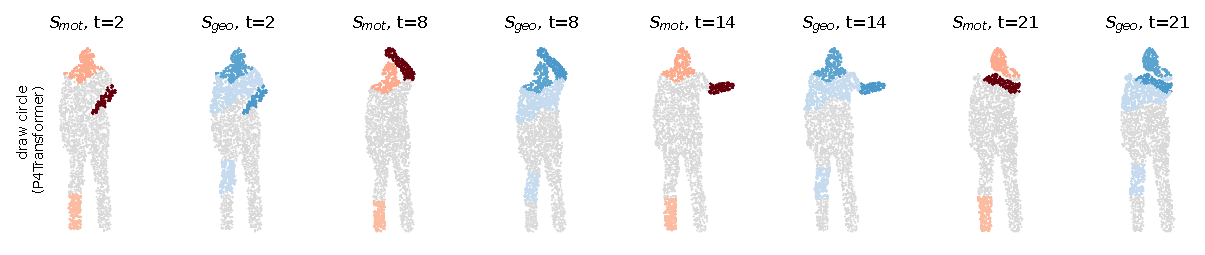
\includegraphics[width=\textwidth]{fig/msr_teaser.pdf}
\caption{\textbf{\methodlong\ (\method)} attributes a 4D model's decision to \emph{how} each spacetime region moves ($\Smot$, red) and to \emph{what shape} it has ($\Sgeo$, blue). It intervenes on the input and reads only the model's output. The clip is a real MSR-Action3D test clip (\emph{draw circle}) at four instants, explained for the official P4Transformer. The motion term is strongest on the drawing hand (weaker on the head and one foot), while geometry importance covers the upper body. Fig.~\ref{fig:qual} in the appendix shows two more actions on all three backbones, including one where the motion term falls on the torso. No attention, gradient or point correspondence is used, and the same code explains convolutional and attention-free state-space backbones (Sec.~\ref{sec:exp-cross}).}
\label{fig:teaser}
\end{figure*}
